\section{Resultados}
    \subsection{Calidad de los datos}
        La primera verificación resultó decisiva. De las 1.065.888 filas
        descargadas, 533.096 (50,01\,\%) son duplicados exactos y el identificador
        \texttt{estu\_consecutivo} tiene solo 532.792 valores distintos: cada
        registro aparece dos veces en la tabla del portal. Tras eliminar los
        duplicados quedan 532.792 estudiantes con identificador único, cifra
        coherente con la población que presenta la prueba en el calendario A. El
        hallazgo no habría alterado las medias, pero sí todos los conteos y, en
        la fase de modelado, habría colocado el mismo estudiante en entrenamiento
        y en prueba, inflando artificialmente cualquier métrica.

        \vspace{10pt}

        {\sloppy\hbadness=5000
        Dos columnas son constantes (\texttt{periodo} y
        \texttt{estu\_estudiante}) y tres casi constantes,
        \texttt{cole\_calendario} (99,58\,\% A, porque los colegios de calendario
        B presentan en el periodo 2022-1), \texttt{estu\_estadoinvestigacion}
        (99,96\,\%) y \texttt{estu\_privado\_libertad} (99,95\,\%). Los códigos
        y nombres del colegio tienen entre 9.412 y 13.748 niveles y los
        municipios más de 1.000, mientras que el departamento tiene 33.
        \par}

        \vspace{10pt}

        Los valores faltantes (Fig.~\ref{missing_values}) se concentran en
        \texttt{cole\_bilingue} (18,0\,\%) y en el bloque del hogar (4,3 a
        6,7\,\%); los puntajes están completos salvo inglés (0,37\,\%). El
        2,31\,\% de los estudiantes no respondió ninguna pregunta del
        cuestionario, el 10,14\,\% tiene al menos una respuesta faltante y el
        89,86\,\% lo diligenció completo. La ausencia no es aleatoria, puesto que
        quienes no tienen cuestionario promedian 229,1 puntos frente a 250,6 de
        quienes sí lo tienen.

        \begin{figure}[H]
            \centerline{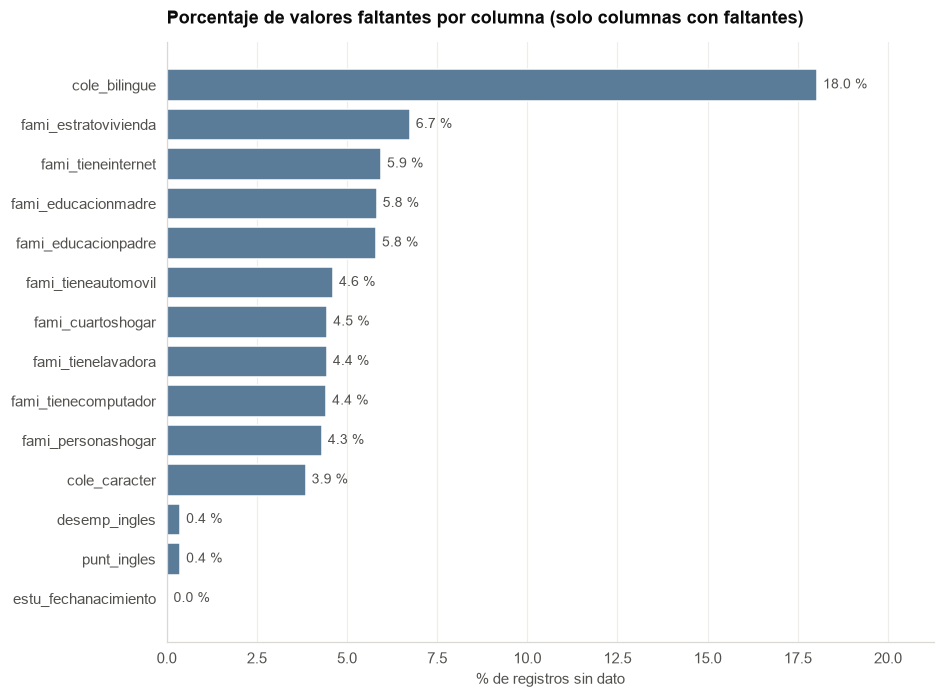
\includegraphics[width=1\linewidth]{assets/images/data/missing_values.png}}
            \caption{Porcentaje de valores faltantes por columna, para las
            columnas que tienen al menos uno.}
            \label{missing_values}
        \end{figure}

        La fecha de nacimiento se convirtió en edad al momento de la prueba, con
        media de 17,8 años, mediana de 17,2 y el 50\,\% central entre 16,7 y 18,1
        años; solo 81 fechas no pudieron interpretarse y 218 edades quedaron
        fuera del rango plausible.

    \subsection{Variable objetivo}
        El puntaje global tiene media de 250,1, mediana de 247 y desviación de
        51,8 puntos; la mitad central de los estudiantes queda entre 210 y 288, el
        1\,\% inferior por debajo de 156 y el 1\,\% superior por encima de 369. La
        asimetría de 0,28 y la curtosis de $-0{,}54$ describen una distribución
        casi simétrica, con una leve cola derecha y colas más ligeras que la
        normal (Fig.~\ref{target_distribution}), de modo que no hace falta
        transformar la variable y las métricas de error se leen directamente en
        puntos.

        \clearpage
        \begin{strip}
            \centering
            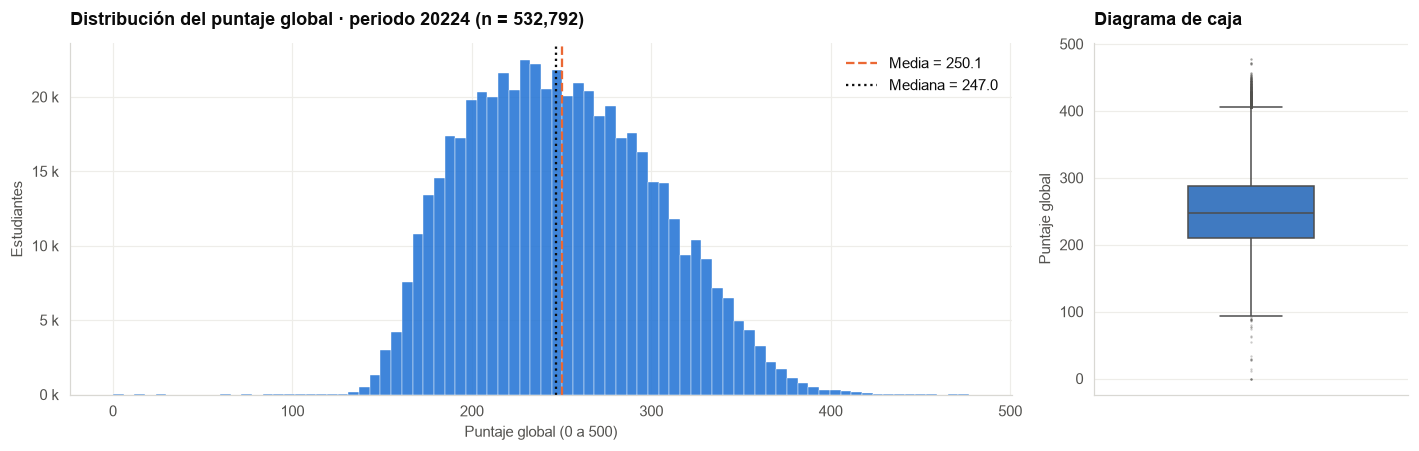
\includegraphics[width=0.98\linewidth]{assets/images/data/target_distribution.png}
            \captionof{figure}{Distribución del puntaje global en el periodo
            2022-4 (532.792 estudiantes): histograma con media y mediana, y
            diagrama de caja.}
            \label{target_distribution}
        \end{strip}

        La fórmula (\ref{global_formula}) se cumple en el 100\,\% de los 530.815
        registros que tienen las cinco pruebas, con una diferencia máxima de cero
        puntos, y cada área correlaciona entre 0,91 y 0,92 con el global (0,80
        inglés). El puntaje global es por tanto una función determinista de los
        puntajes por área, y estos quedan excluidos del conjunto de variables
        explicativas.

    \subsection{Variables del estudiante}
        Los hombres promedian 254,1 puntos y las mujeres 246,8, una brecha de 7,3
        puntos. La edad es una de las variables más informativas
        (Fig.~\ref{student_variables}): los estudiantes de 16 y 17 años promedian
        265 puntos, a los 18 el promedio baja a 250,5, a los 19 y 20 a 229,5,
        entre 21 y 25 a 206,1 y de 26 en adelante a 199,6, una caída de más de 65
        puntos que marca trayectorias de extraedad y educación de adultos. El tipo
        de documento redunda con la edad, la tarjeta de identidad promedia 255,6
        y la cédula de ciudadanía 219,4.

        \begin{strip}
            \centering
            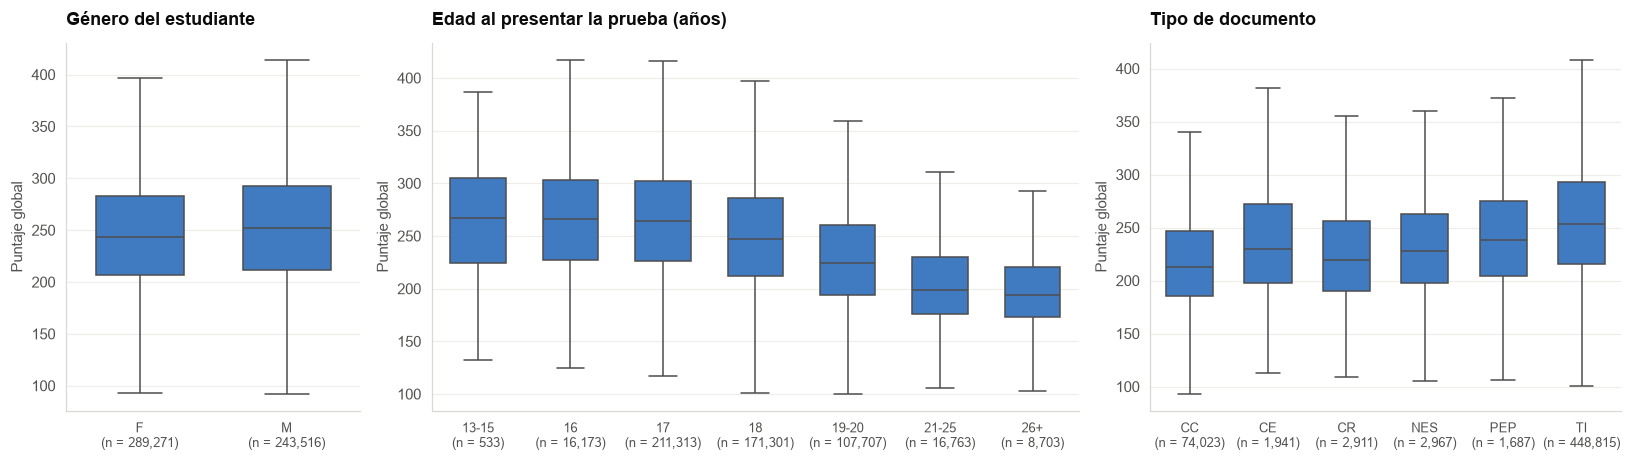
\includegraphics[width=0.98\linewidth]{assets/images/data/student_variables.png}
            \captionof{figure}{Puntaje global según género, tramo de edad y tipo
            de documento del estudiante (diagramas de caja sin valores atípicos;
            $n$ de cada grupo en el eje).}
            \label{student_variables}
        \end{strip}

    \subsection{Variables del hogar}
        La Tabla~\ref{family_table} y la Fig.~\ref{family_ordinal} muestran la
        gradiente socioeconómica. La educación de la madre tiene una relación
        perfectamente monótona con el puntaje, de 211,2 puntos cuando no tiene
        ningún nivel educativo a 307,5 cuando tiene posgrado, 96 puntos de
        diferencia, el contraste más amplio del análisis; la del padre va de 214,5
        a 311,9, y su categoría \textit{No sabe} reúne 36.317 estudiantes
        (6,8\,\%), reflejo de hogares sin presencia paterna, que promedian 260,7.
        El estrato sube de 212,6 (\textit{Sin estrato}) a 267,4 (estrato 4) pero
        cae en los estratos 5 (261,4) y 6 (245,1), que tienen las desviaciones
        más altas y los grupos más pequeños, un quiebre que apunta a errores de
        reporte en el cuestionario.

        \begin{table}[H]
            \centering
            \caption{Puntaje global medio según variables ordinales del hogar}
            \label{family_table}
            \begin{tabular}{|l|r|r|}
                \hline
                \textbf{Variable y nivel} & \textbf{$n$} & \textbf{Media} \\
                \hline
                Estrato: Sin estrato & 19.781 & 212,6 \\
                \hline
                Estrato 1 & 146.333 & 242,0 \\
                \hline
                Estrato 2 & 180.091 & 253,7 \\
                \hline
                Estrato 3 & 110.254 & 263,2 \\
                \hline
                Estrato 4 & 28.092 & 267,4 \\
                \hline
                Estrato 5 & 8.448 & 261,4 \\
                \hline
                Estrato 6 & 3.879 & 245,1 \\
                \hline
                Educ. madre: Ninguno & 10.260 & 211,2 \\
                \hline
                Primaria completa & 42.124 & 233,4 \\
                \hline
                Secundaria completa & 143.736 & 249,4 \\
                \hline
                Técnica o tecnológica completa & 52.289 & 268,0 \\
                \hline
                Educación profesional completa & 62.318 & 278,4 \\
                \hline
                Postgrado & 11.372 & 307,5 \\
                \hline
                No sabe & 12.638 & 261,5 \\
                \hline
            \end{tabular}
        \end{table}

        \clearpage
        \begin{strip}
            \centering
            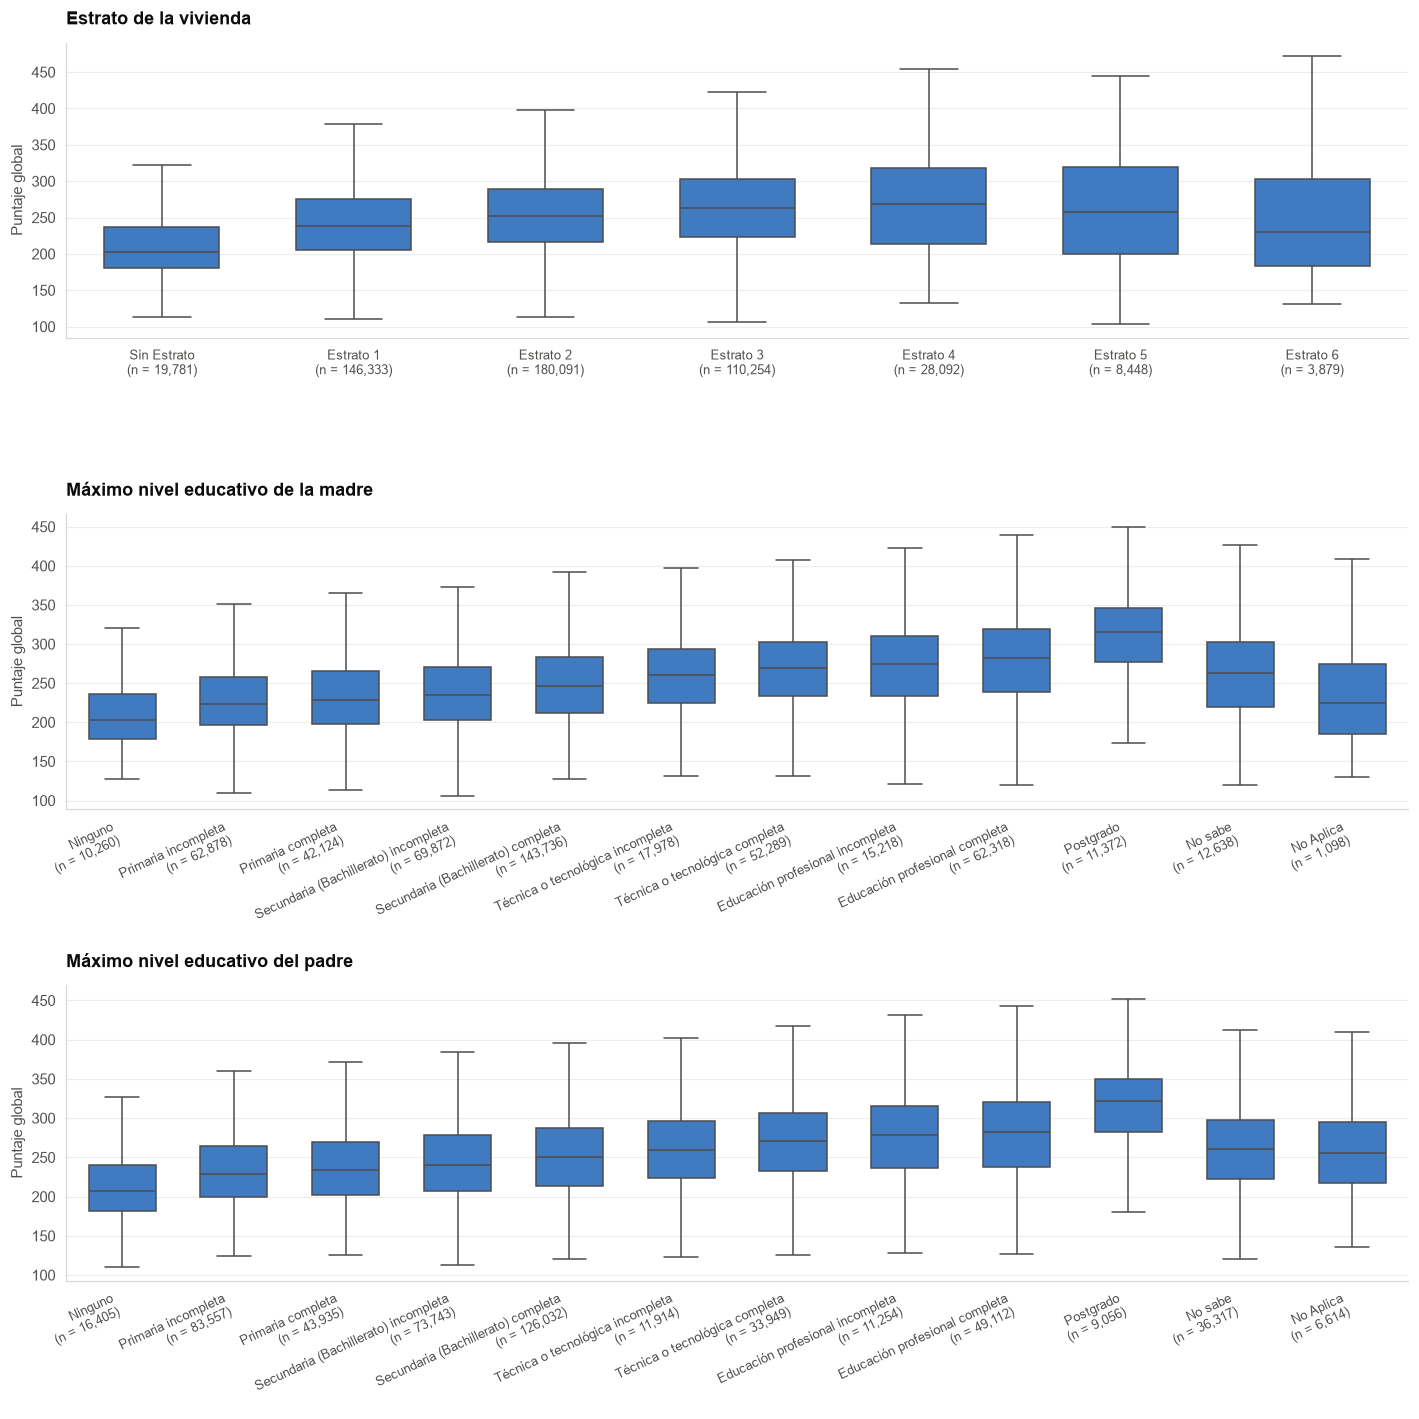
\includegraphics[width=0.78\linewidth]{assets/images/data/family_ordinal.png}
            \captionof{figure}{Puntaje global según estrato de la vivienda y
            máximo nivel educativo de la madre y del padre.}
            \label{family_ordinal}
        \end{strip}

        Tener internet (+31,8 puntos) y computador (+31,7) marcan una diferencia
        muy superior a la del automóvil (+23,6) y la lavadora (+20,8), y en 2022
        todavía el 27\,\% de los hogares declaraba no tener internet. La
        composición del hogar no es monótona (Fig.~\ref{family_binary}): el
        puntaje es máximo en hogares de 3 a 4 personas (257,1) y en viviendas de
        tres cuartos (255,8), y desciende hacia ambos extremos, hasta 225,0 en
        hogares de 9 o más personas y 232,3 en viviendas de seis o más cuartos,
        frecuentes en zonas rurales de bajo ingreso.

        \begin{strip}
            \centering
            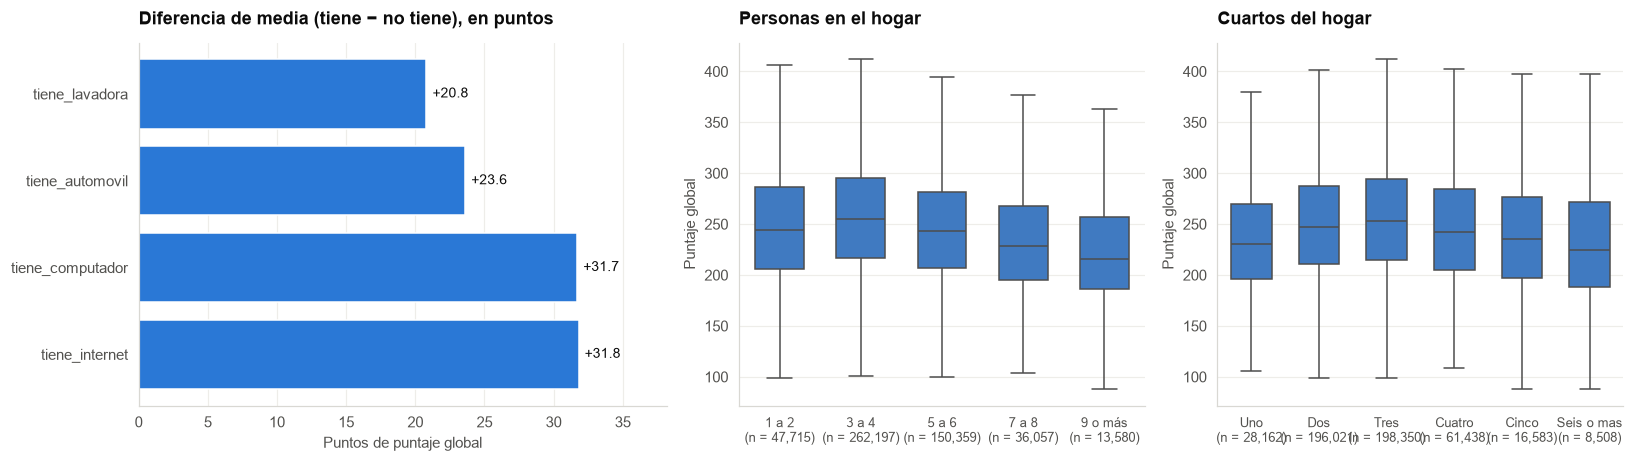
\includegraphics[width=0.98\linewidth]{assets/images/data/family_binary.png}
            \captionof{figure}{Diferencia de puntaje medio según tenencia de
            bienes del hogar, y puntaje según personas y cuartos del hogar.}
            \label{family_binary}
        \end{strip}

    \subsection{Variables del colegio}
        La Tabla~\ref{school_table} y la Fig.~\ref{school_variables} resumen las
        variables del colegio. Los colegios no oficiales promedian 272,6 puntos
        frente a 243,6 de los oficiales (29 puntos), los urbanos 254,6 frente a
        228,4 de los rurales (26,2 puntos), y la jornada es la variable con mayor
        rango: la completa promedia 280,8 mientras que la sabatina (212,7) y la
        nocturna (210,6) quedan 70 puntos por debajo. El carácter académico
        (253,9) supera levemente al técnico (243,3). Contra lo esperado, los
        colegios marcados como bilingües promedian 247,0, por debajo de los no
        bilingües (252,1), lo que sumado a su 18\,\% de faltantes hace del
        indicador una variable poco confiable. Los colegios femeninos (285,5) y
        masculinos (294,2) superan por mucho a los mixtos (249,0), pero son grupos
        pequeños compuestos sobre todo por colegios privados.

        \begin{table}[H]
            \centering
            \caption{Puntaje global medio según variables del colegio}
            \label{school_table}
            \begin{tabular}{|l|r|r|}
                \hline
                \textbf{Variable y nivel} & \textbf{$n$} & \textbf{Media} \\
                \hline
                Naturaleza: Oficial & 412.313 & 243,6 \\
                \hline
                No oficial & 120.478 & 272,6 \\
                \hline
                Área: Urbano & 441.577 & 254,6 \\
                \hline
                Rural & 91.214 & 228,4 \\
                \hline
                Jornada: Completa & 76.897 & 280,8 \\
                \hline
                Única & 146.360 & 252,0 \\
                \hline
                Mañana & 208.530 & 248,2 \\
                \hline
                Tarde & 49.187 & 245,5 \\
                \hline
                Sabatina & 28.116 & 212,7 \\
                \hline
                Noche & 23.701 & 210,6 \\
                \hline
                Carácter: Académico & 269.918 & 253,9 \\
                \hline
                Técnico/académico & 174.947 & 248,9 \\
                \hline
                Técnico & 58.697 & 243,3 \\
                \hline
            \end{tabular}
        \end{table}

        \clearpage
        \begin{strip}
            \centering
            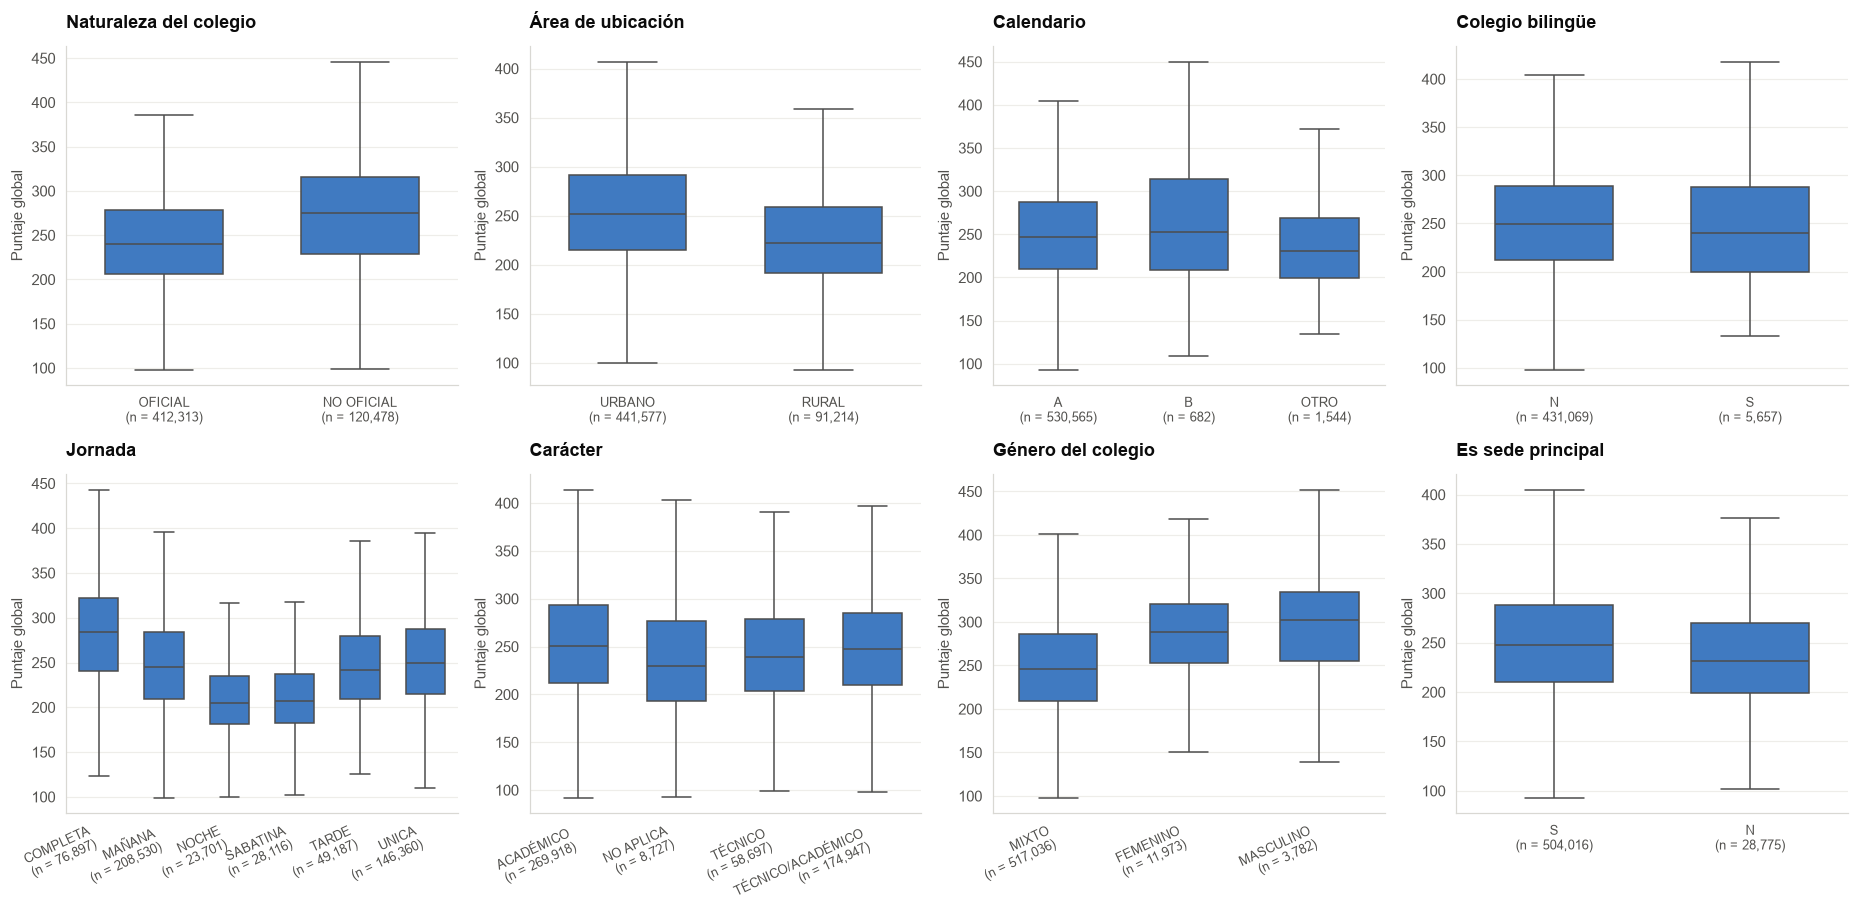
\includegraphics[width=0.98\linewidth]{assets/images/data/school_variables.png}
            \captionof{figure}{Puntaje global según naturaleza, área,
            calendario, bilingüismo, jornada, carácter, género y sede del
            colegio.}
            \label{school_variables}
        \end{strip}

        El cruce entre naturaleza y área (Tabla~\ref{crosstab}) desenreda ambos
        efectos. Entre los colegios oficiales la brecha urbano-rural es de 24
        puntos, pero entre los no oficiales se invierte: los privados rurales,
        pocos y en buena parte colegios campestres, promedian 291,1, el valor más
        alto de las cuatro celdas. Un modelo lineal necesitará un término de
        interacción entre ambas variables.

        \begin{table}[H]
            \centering
            \caption{Puntaje global medio y tamaño según naturaleza y área del colegio}
            \label{crosstab}
            \begin{tabular}{|l|r|r|r|r|}
                \hline
                & \multicolumn{2}{c|}{\textbf{Media}} & \multicolumn{2}{c|}{\textbf{$n$}} \\
                \hline
                \textbf{Naturaleza} & Rural & Urbano & Rural & Urbano \\
                \hline
                No oficial & 291,1 & 271,7 & 5.328 & 115.150 \\
                \hline
                Oficial & 224,5 & 248,6 & 85.886 & 326.427 \\
                \hline
            \end{tabular}
        \end{table}

    \subsection{Variables geográficas}
        La brecha regional es grande y ordenada (Fig.~\ref{geography}). Bogotá
        (270,2), Boyacá (268,6), Santander (267,0) y Cundinamarca (262,8)
        encabezan la lista; Chocó (206,1), Vaupés (213,7), Amazonas (215,5),
        Vichada (217,9) y La Guajira (221,5) la cierran. Entre el primero y el
        último hay 64,1 puntos, más que la diferencia entre colegios oficiales y
        privados, y solo 11 de los 33 departamentos superan la media nacional de
        250,1. Varios departamentos tienen muy pocos estudiantes (Guainía 389,
        Vaupés 434, San Andrés 577), lo que exige una codificación regularizada.

        \begin{figure}[H]
            \centerline{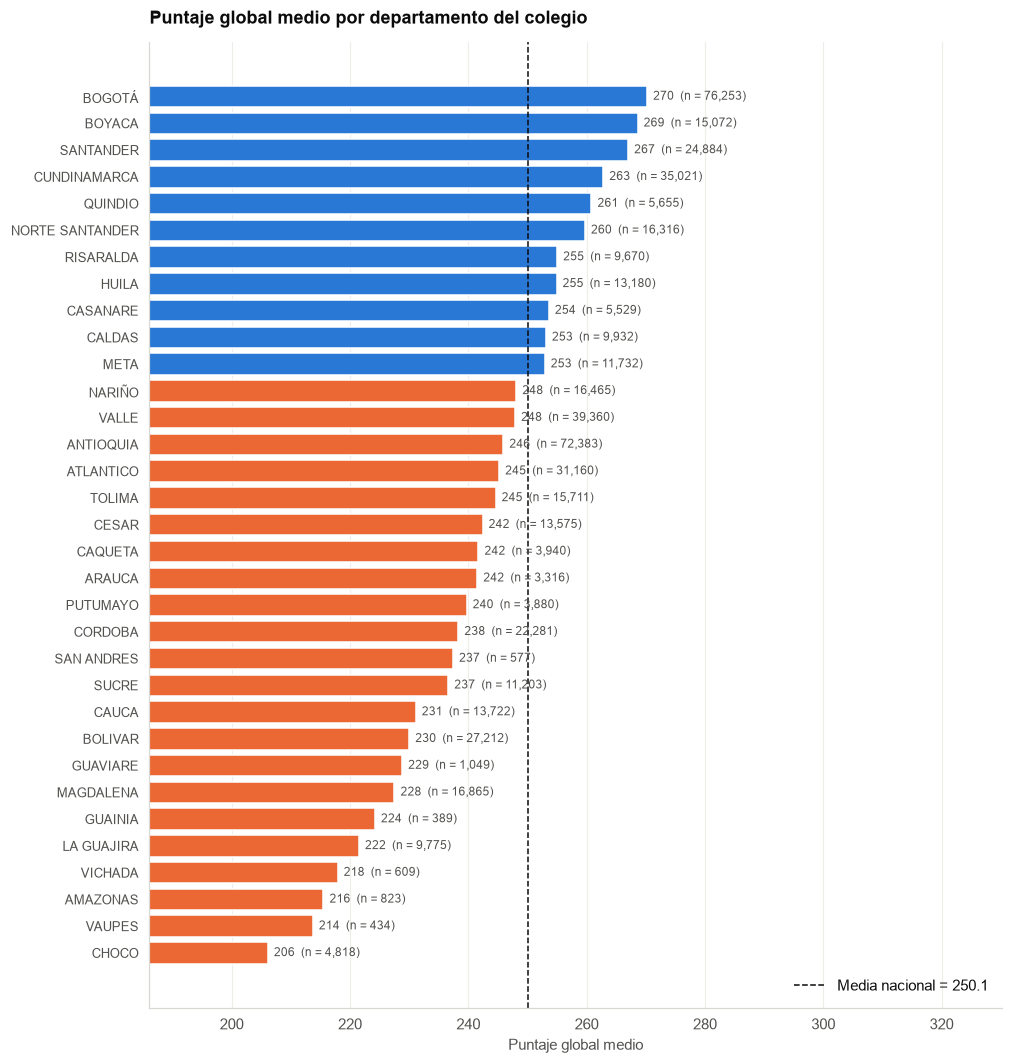
\includegraphics[width=1\linewidth]{assets/images/data/geography.png}}
            \caption{Puntaje global medio por departamento del colegio; en azul
            los departamentos por encima de la media nacional y en naranja los
            que están por debajo.}
            \label{geography}
        \end{figure}

    \subsection{Correlaciones y ajuste lineal exploratorio}
        La matriz de correlación de Spearman (Fig.~\ref{correlation_matrix})
        muestra el contraste buscado, los puntajes por área correlacionan entre
        0,91 y 0,92 con el global mientras que ninguna variable explicativa
        legítima supera 0,35 (Tabla~\ref{spearman_table}). Las variables del hogar
        están además correlacionadas entre sí (educación de la madre y del padre
        0,61; computador e internet 0,48), de modo que miden facetas del mismo
        nivel socioeconómico.

        \begin{table}[H]
            \centering
            \caption{Correlación de Spearman de las variables candidatas con el puntaje global}
            \label{spearman_table}
            \begin{tabular}{|l|r|}
                \hline
                \textbf{Variable} & $\boldsymbol{\rho}$ \\
                \hline
                Educación de la madre & 0,35 \\
                \hline
                Edad & $-$0,32 \\
                \hline
                Educación del padre & 0,32 \\
                \hline
                Tiene computador & 0,30 \\
                \hline
                Tiene internet & 0,28 \\
                \hline
                Colegio no oficial & 0,22 \\
                \hline
                Estrato & 0,19 \\
                \hline
                Colegio urbano & 0,19 \\
                \hline
                Jornada completa o única & 0,19 \\
                \hline
                Tiene automóvil & 0,19 \\
                \hline
                Tiene lavadora & 0,17 \\
                \hline
                Personas en el hogar & $-$0,11 \\
                \hline
                Género femenino & $-$0,07 \\
                \hline
                Colegio bilingüe, cuartos, calendario B & $|\rho| \le 0{,}01$ \\
                \hline
            \end{tabular}
        \end{table}

        \clearpage
        \begin{strip}
            \centering
            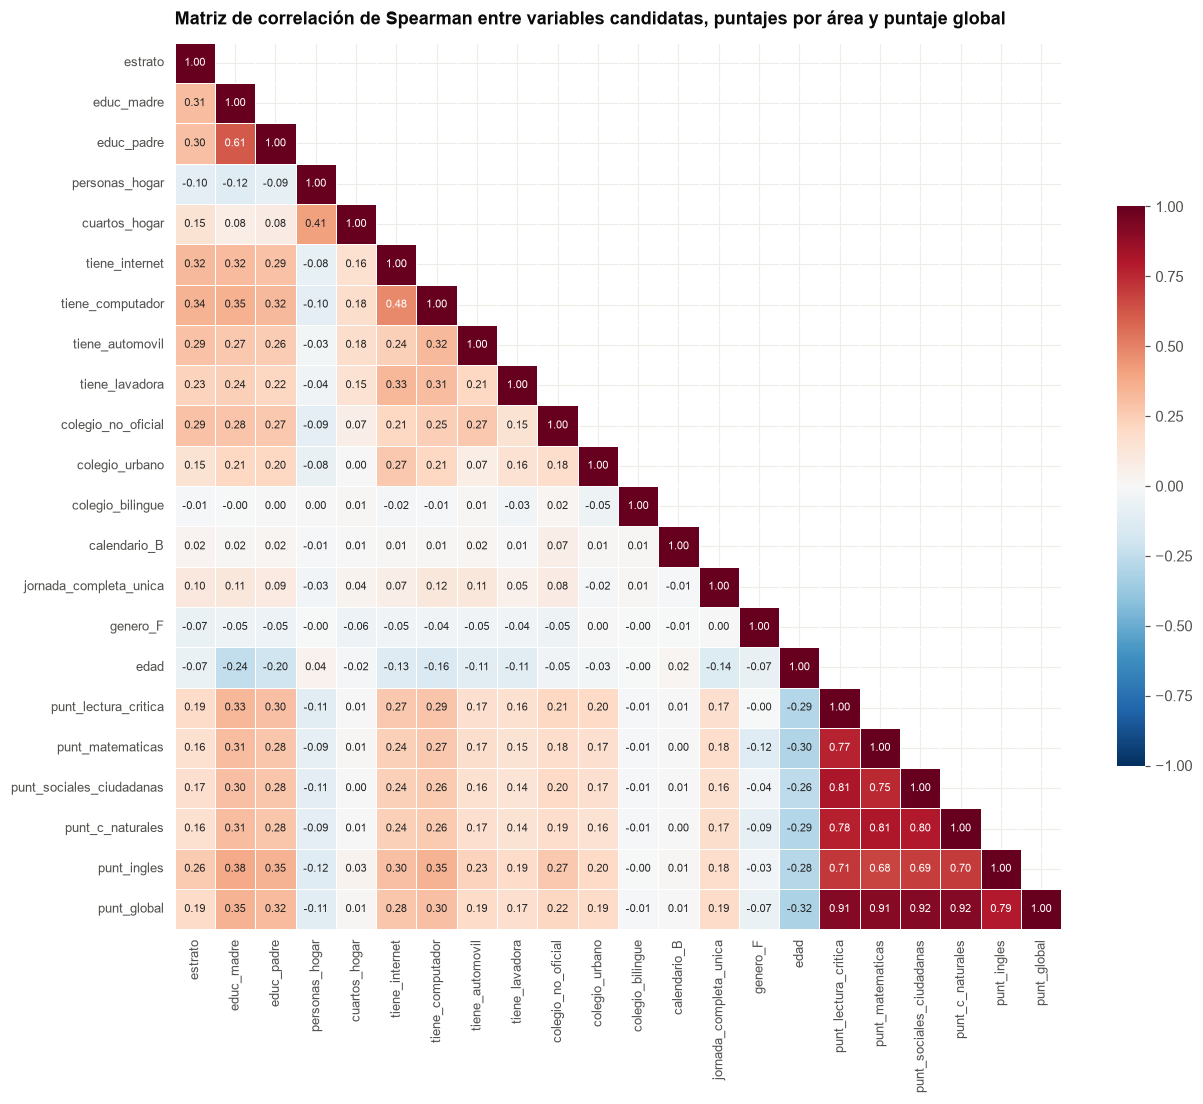
\includegraphics[width=0.72\linewidth]{assets/images/data/correlation_matrix.png}
            \captionof{figure}{Matriz de correlación de Spearman entre las
            variables candidatas codificadas, los puntajes por área y el puntaje
            global.}
            \label{correlation_matrix}
        \end{strip}

        Una regresión lineal sobre las variables codificadas, con 200.000 filas
        completas y partición 80/20, alcanza un $R^2$ de 0,242 y un MAE de 36,5
        puntos frente a 42,6 de predecir siempre la media, una reducción del
        14\,\%. Los coeficientes ratifican los resultados bivariados: colegio no
        oficial (+14,4 puntos), computador (+11,4), jornada completa o única
        (+11,1), internet (+10,1) y colegio urbano (+9,3) son los mayores efectos
        por unidad; cada nivel educativo de la madre suma 3,0 puntos y cada año
        de edad resta 2,9. El estrato queda con un coeficiente casi nulo
        ($-0{,}56$) porque los bienes del hogar y la educación de los padres
        absorben su información.

    \subsection{Hallazgos y decisiones para la fase 2}
        Los hallazgos anteriores se traducen en las decisiones de preparación de
        datos e ingeniería de variables de la Tabla~\ref{decisions}. Con ellas, el
        conjunto de trabajo para la fase 2 queda en 532.792 registros y cerca de
        22 variables explicativas, con el puntaje global como objetivo.

        \clearpage
        \begin{strip}
            \centering
            \captionof{table}{Hallazgos del análisis exploratorio y decisiones para la fase 2}
            \label{decisions}
            \small
            \begin{tabular}{|L{7.6cm}|L{9.6cm}|}
                \hline
                \textbf{Hallazgo} & \textbf{Decisión} \\
                \hline
                Cada registro aparece dos veces & Eliminar duplicados antes de particionar. \\
                \hline
                El global es función exacta de las áreas & Excluir \texttt{punt\_*} por área y \texttt{desemp\_ingles}. \\
                \hline
                La ausencia del cuestionario es informativa (21,5 puntos menos) & Conservar faltantes como categoría \textit{no respondió} e indicador de cuestionario incompleto. \\
                \hline
                Columnas constantes, casi constantes, identificadores y nombres & Descartarlas; conservar departamento y municipio del colegio. \\
                \hline
                Educación de los padres e internet/computador lideran & Educación como ordinal 0 a 9 con \textit{No sabe} como nivel propio; bienes binarios. \\
                \hline
                El estrato se quiebra en 5 y 6 & Probarlo como nominal o agrupar 4 a 6. \\
                \hline
                Personas y cuartos en forma de U & Crear personas por cuarto; tratarlas como categóricas. \\
                \hline
                La edad marca extraedad & Edad numérica e indicador de extraedad; descartar tipo de documento. \\
                \hline
                Jornada, naturaleza y área con interacción & Nominales más interacción naturaleza $\times$ área. \\
                \hline
                Indicador bilingüe poco confiable & Descartarlo o conservarlo con \textit{no reportado}. \\
                \hline
                Brecha regional con departamentos pequeños & \textit{One-hot} o codificación por objetivo suavizada; municipio solo por objetivo. \\
                \hline
                $R^2$ lineal de 0,242 & Referencia: regresión lineal regularizada; meta de la fase 3: superarla con modelos no lineales. \\
                \hline
            \end{tabular}
        \end{strip}
